\documentclass[11pt]{article}
\usepackage[a4paper, total={6.5in, 9.4in}]{geometry}
\usepackage{graphicx}
\graphicspath{ {./images/output/} }
\usepackage{caption}
\usepackage[english]{babel}
\usepackage{titling}
\usepackage{float}
\usepackage{amsmath}
\usepackage{minted}
\usepackage{multicol}
\usepackage{array}
\usepackage{setspace}
\usepackage{placeins}

\usepackage{parskip}

% \usepackage{lipsum}

\title{Performing DFT to Compute Convulation Between Two Signals}
\author{}
\date{}

\pagenumbering{gobble}
\begin{document}
\vspace*{\fill}
\begin{center}

    \emph{Heaven's Light is Our Guide} \\
    \textbf{Rajshahi University of Engineering and Technology} \\

    \begin{figure}[H]
        \centering
        
\includegraphics[scale=.34]{images/RUET_logo.png}
        \label{fig:ruet_logo}
    \end{figure}
    \vspace{5mm}

    \textbf{Course Code}\\
    ECE 4124\\
    \vspace{3mm}
    \textbf{Course Title}\\
    Digital Signal Processing Sessional

    \vspace{5mm}
    \textbf{Experiment Date:} {September 13, 2025}\\
    \textbf{Submission Date:} {October 11, 2025}\\

    \vspace{5mm}
    \textbf{Lab Report 4: \\
        Performing DFT to compute Convulation Between Two Signals}

    \vspace{15mm}

    \begin{tabular}{c|c}
        \textbf{Submitted to} & \textbf{Submitted by} \\
        Md. Faysal Ahamed     &                       \\
        Assistant Professor   &                       \\
        Dept of ECE, RUET     & Md. Tajim An Noor     \\
        \&                    & Roll: 2010025         \\
        Moloy Kumar Ghosh     &                       \\
        Lecturer              &                       \\
        Dept of ECE, RUET     &                       \\
    \end{tabular}

\end{center}
\vspace*{\fill}


\pagebreak

\tableofcontents

\pagebreak
\pagenumbering{arabic}
\maketitle

\section*{Theory}
\addcontentsline{toc}{section}{Theory}

\subsection*{Direct Convolution}
\addcontentsline{toc}{subsection}{Direct Convolution}
Convolution is a mathematical operation used to combine two signals to produce a third signal that expresses how the shape of one is modified by the other. In discrete-time signal processing, the convolution of two sequences $x[n]$ and $h[n]$ is defined as:
\begin{equation}
    y[n] = (x * h)[n] = \sum_{k=0}^{N-1} x[k] \cdot h[n-k]
\end{equation}
where $N$ is the length of the sequences. This process involves sliding one signal over another, multiplying and summing the overlapping values~\cite{oppenheim1999discrete}.

\textbf{Process:}
\begin{enumerate}
    \item Reverse one of the sequences (usually $h[n]$).
    \item Shift it across the other sequence ($x[n]$).
    \item For each shift, multiply overlapping values and sum them to get each output value.
\end{enumerate}

\textbf{Example:}
Let $x[n] = [1, 2, 3]$ and $h[n] = [4, 5]$. The convolution is:
\begin{align*}
    y[0] & = 1 \cdot 4 = 4                        \\
    y[1] & = 1 \cdot 5 + 2 \cdot 4 = 5 + 8 = 13   \\
    y[2] & = 2 \cdot 5 + 3 \cdot 4 = 10 + 12 = 22 \\
    y[3] & = 3 \cdot 5 = 15
\end{align*}
So, $y[n] = [4, 13, 22, 15]$.


\subsection*{Convolution Using DFT}
\addcontentsline{toc}{subsection}{Convulation Using DFT}
Convolution can also be performed using the Discrete Fourier Transform (DFT) due to the Convolution Theorem, which states that convolution in the time domain corresponds to multiplication in the frequency domain~\cite{proakis2007digital}.

\textbf{Process:}
\begin{enumerate}
    \item Zero-pad both sequences to the same length (usually $N = N_x + N_h - 1$).
    \item Compute the DFT of both sequences: $X[k] = \text{DFT}(x[n])$, $H[k] = \text{DFT}(h[n])$.
    \item Multiply the DFTs pointwise: $Y[k] = X[k] \cdot H[k]$.
    \item Compute the inverse DFT (IDFT) of $Y[k]$ to obtain the convolution result in the time domain.
\end{enumerate}

\textbf{Example:}
Given $x[n] = [1, 2, 3]$ and $h[n] = [4, 5]$, zero-pad both to length $4$:
\begin{align*}
    x[n] & = [1, 2, 3, 0] \\
    h[n] & = [4, 5, 0, 0]
\end{align*}
Compute DFTs, multiply, and take IDFT to get $y[n] = [4, 13, 22, 15]$ (same as direct convolution).


\textbf{Summary:} Direct convolution is straightforward for short signals, while DFT-based convolution is efficient for long signals due to fast algorithms like FFT~\cite{oppenheim1999discrete,proakis2007digital}.

\section*{Used Tools}
\addcontentsline{toc}{section}{Used Tools}
\begin{itemize}
    \item Matlab Online
    \item LaTex
\end{itemize}

\section*{Code \& Output}
\addcontentsline{toc}{section}{Code \& Output}

\subsection*{Code}
\addcontentsline{toc}{subsection}{Code}
\begin{multicols}{2}
    \inputminted[fontsize=\small, linenos, breaklines]{matlab}{assets/dft.m}
\end{multicols}

\subsection*{Output}
\addcontentsline{toc}{subsection}{Output}
\begin{figure}[H]
    \centering
    \begin{minted}[fontsize=\small]{text}
Convolution using DFT:
  -10.0000   28.0000  -10.0000    3.0000   29.0000  -16.0000   11.0000    5.0000   -0.0000

Direct convolution:
   -10    28   -10     3    29   -16    11     5     0
    \end{minted}
    \caption{Console Output}
\end{figure}

\begin{figure}[H]
    \centering
    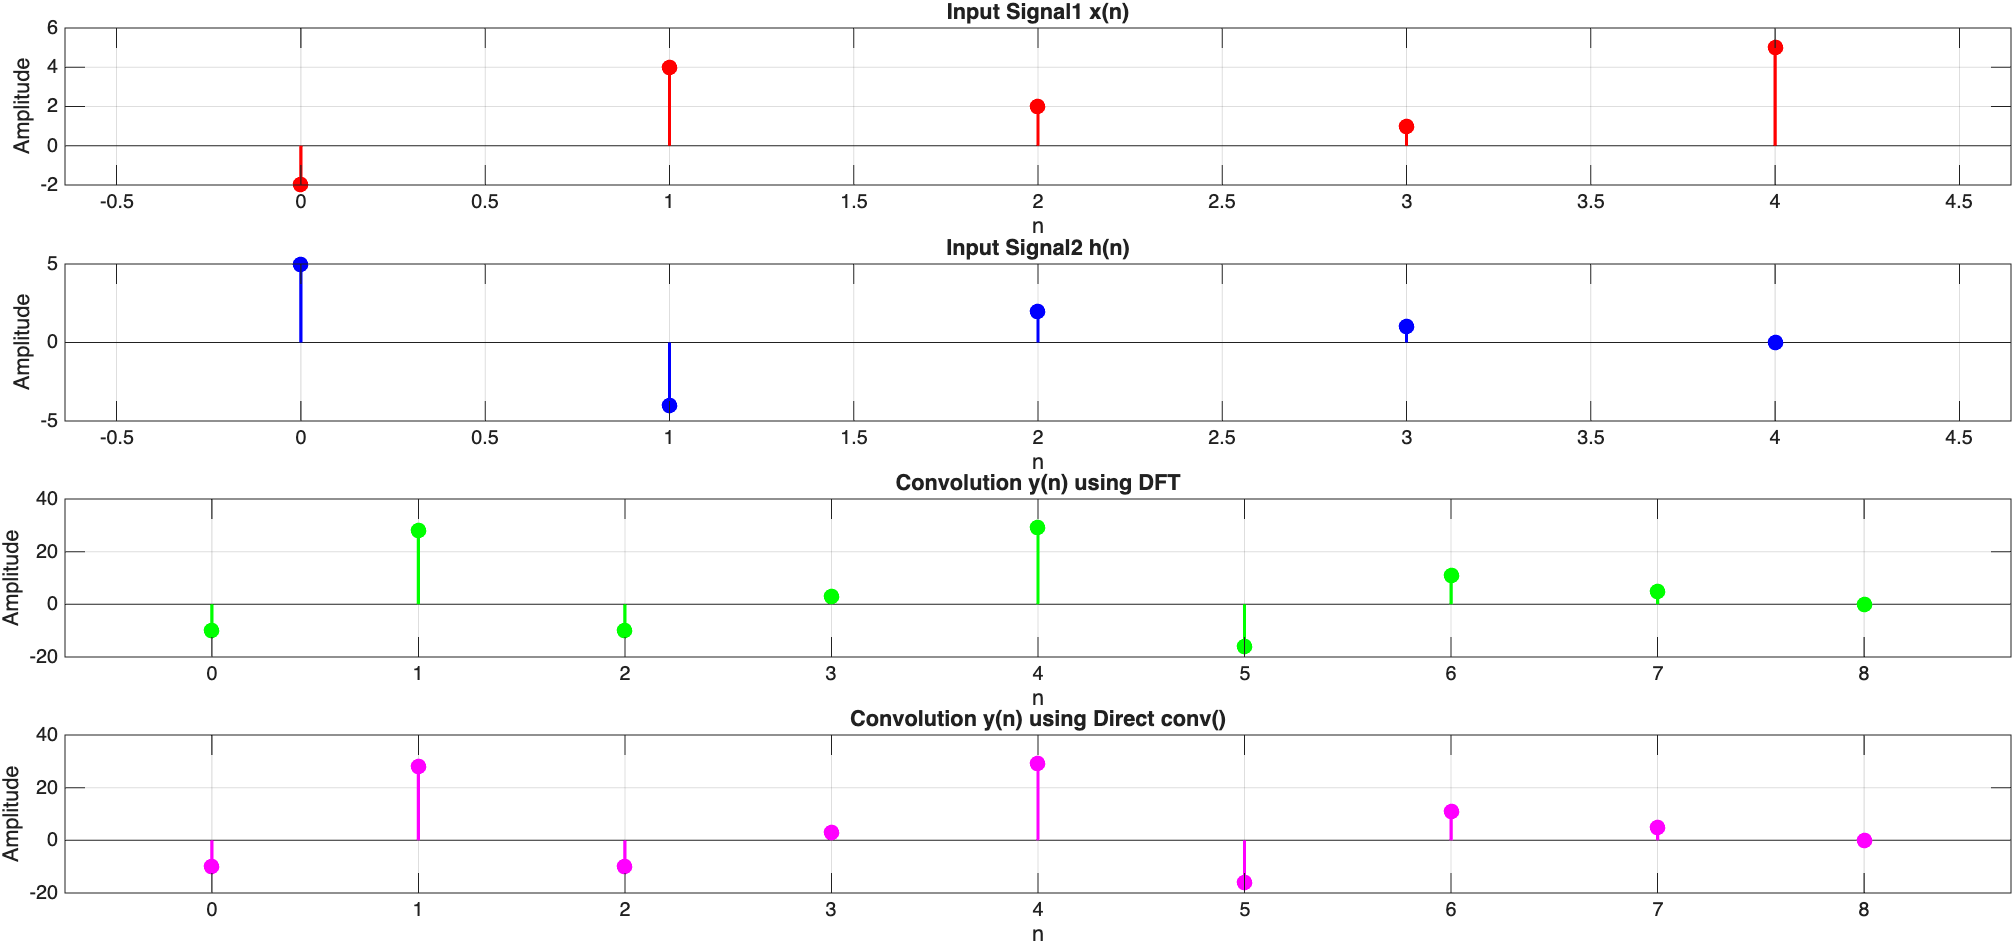
\includegraphics[width=\textwidth]{plot.png}
    \caption{Plot Output}
\end{figure}

\section*{Discussion}
\addcontentsline{toc}{section}{Discussion}
In this experiment, the convolution of two discrete signals was computed using both the direct method and the DFT-based approach. The results obtained from both methods were observed to be identical, confirming the validity of the Convolution Theorem. The DFT-based method was facilitated by zero-padding the input sequences, transforming them into the frequency domain, performing pointwise multiplication, and then applying the inverse DFT. The efficiency of the DFT-based convolution was highlighted, especially for longer signals, where computational advantages were realized due to the use of FFT algorithms. The outputs and plots generated by Matlab were used to verify the correctness of the implementation.

\section*{Conclusion}
\addcontentsline{toc}{section}{Conclusion}
The convolution between two signals was successfully performed using both direct computation and the DFT-based method. The equivalence of the results demonstrated the practical application of the Convolution Theorem in digital signal processing. The experiment illustrated that while direct convolution is suitable for short signals, the DFT-based approach is preferred for longer signals due to its computational efficiency. The use of Matlab and LaTeX facilitated the analysis and presentation of the results.

\bibliographystyle{IEEEtran}
\renewcommand{\bibname}{References}
\addcontentsline{toc}{section}{References}
\bibliography{ref}

\end{document}
